\documentclass[main]{subfiles}

\begin{document}


\chapter{Pruebas del controlador}
El controlador diseñado se comporta adecuadamente en lo que respecta a las simulaciones, sin embargo debido a que la caracterizaci\'on del sistema puede contener errores se proceden a realizar algunas pruebas sobre los subsistemas que componen al sistema global. Estas pruebas son de utilidad para verificar el correcto funcionamiento del controlador diseñado y/o para realizar los ajustes que sean necesarios en el mismo.

\section{Control del subsistema del Roll}

Para lograr el correcto funcionamiento del cuadric\'optero es fundamental que el control sobre los \'angulos de Pitch y de Roll se comporte de buena forma. A modo de ejemplo, es imposible lograr el equilibrio mec\'anico si dichos \'angulos difieren de cero. Por dicha raz\'on, previo a realizar pruebas sobre el sistema completo es necesario asegurarnos que los subsistemas del  Roll y del Pitch funcionan correctamente. De acuerdo al modelo f\'isico del sistema desarrollado en \ref{chap:modelo_fisico} ni el Roll ni el Pitch son subsistemas independientes entre s\'i, adem\'as ambos dependen de la velocidad angular seg\'un $\vec{k}_q$. Sin embargo, dichos \'angulos toman valores cercanos a cero en las trayectorias de inter\'es, en este caso se puede realizar la aproximaci\'on de que ambos sistemas son independientes.\\

\begin{wrapfigure}{r}{0.55\textwidth}
	\vspace{-20pt}
	\centering
	\includegraphics[width=0.4\textwidth]{./pics_test_control/dispositivo_psi.pdf}
	\caption{Dispositivo de prueba de Roll}
	\label{fig:psidisp}
\end{wrapfigure}

A partir de esta consideraci\'on se procede a fijar al cuadric\'optero sobre dos gu\'ias como se muestra en la figura \ref{fig:psidisp}, de forma de eliminar todos los grados de libertad del sistema excepto el \'angulo de Roll y la velocidad angular correspondiente al eje de rotaci\'on del Roll. Se realizan dos pruebas: la primera consiste en que el sistema alcance la posic\'on de equilibrio ($\psi = 0$), la segunda consiste en alejar al sistema del equilibrio y lograr que vuelva al punto de equilibrio. 

\subsection{Equilibrio}
A partir de la matriz determinada originalmente en las simulaciones se realizaron algunas modificaciones a efectos de lograr una performance m\'as adecuada del sistema. En lo que respecta al control del \'angulo en cuesti\'on la relaci\'on entre el coeficiente de la matriz \ref{eq:Qlqr}

\section{Control del subsistema del Yaw}


De manera an\'aloga al caso anterior, es importante verificar el buen funcionamiento del control sobre el giro en ``z'', para lo cual se utiliza un dispositivo de prueba que restringe los grados de libertad del cuadric\'optero. En este caso se lo sujeta con una cuerda desde arriba de los cuatro brazos de modo de realizar la fuerza lo m\'as pareja posible. El cuadric\'optero queda sujetado colgando horizontal y conserva el libre giro seg\'un ``z'' ($\theta$).
Se setea una velocidad de \emph{hovering} inferior a la necesaria para levantar vuelo, de modo que el cuadric\'optero no se eleve y la cuerda quede siempre tensa. Para el giro bajo estudio no es relevante el valor absoluto de la velocidad de giro de cada motor, ya que depende exclusivamente de la diferencia de velocidades angulares. Por ello los resultados de realizar las pruebas con una velocidad de \emph{hovering} inferior a la real son extrapolables a la situaci\'on de vuelo libre, sin p\'erdida de generalidad.\\

\begin{wrapfigure}{r}{0.55\textwidth}
	\vspace{-20pt}
	\centering
	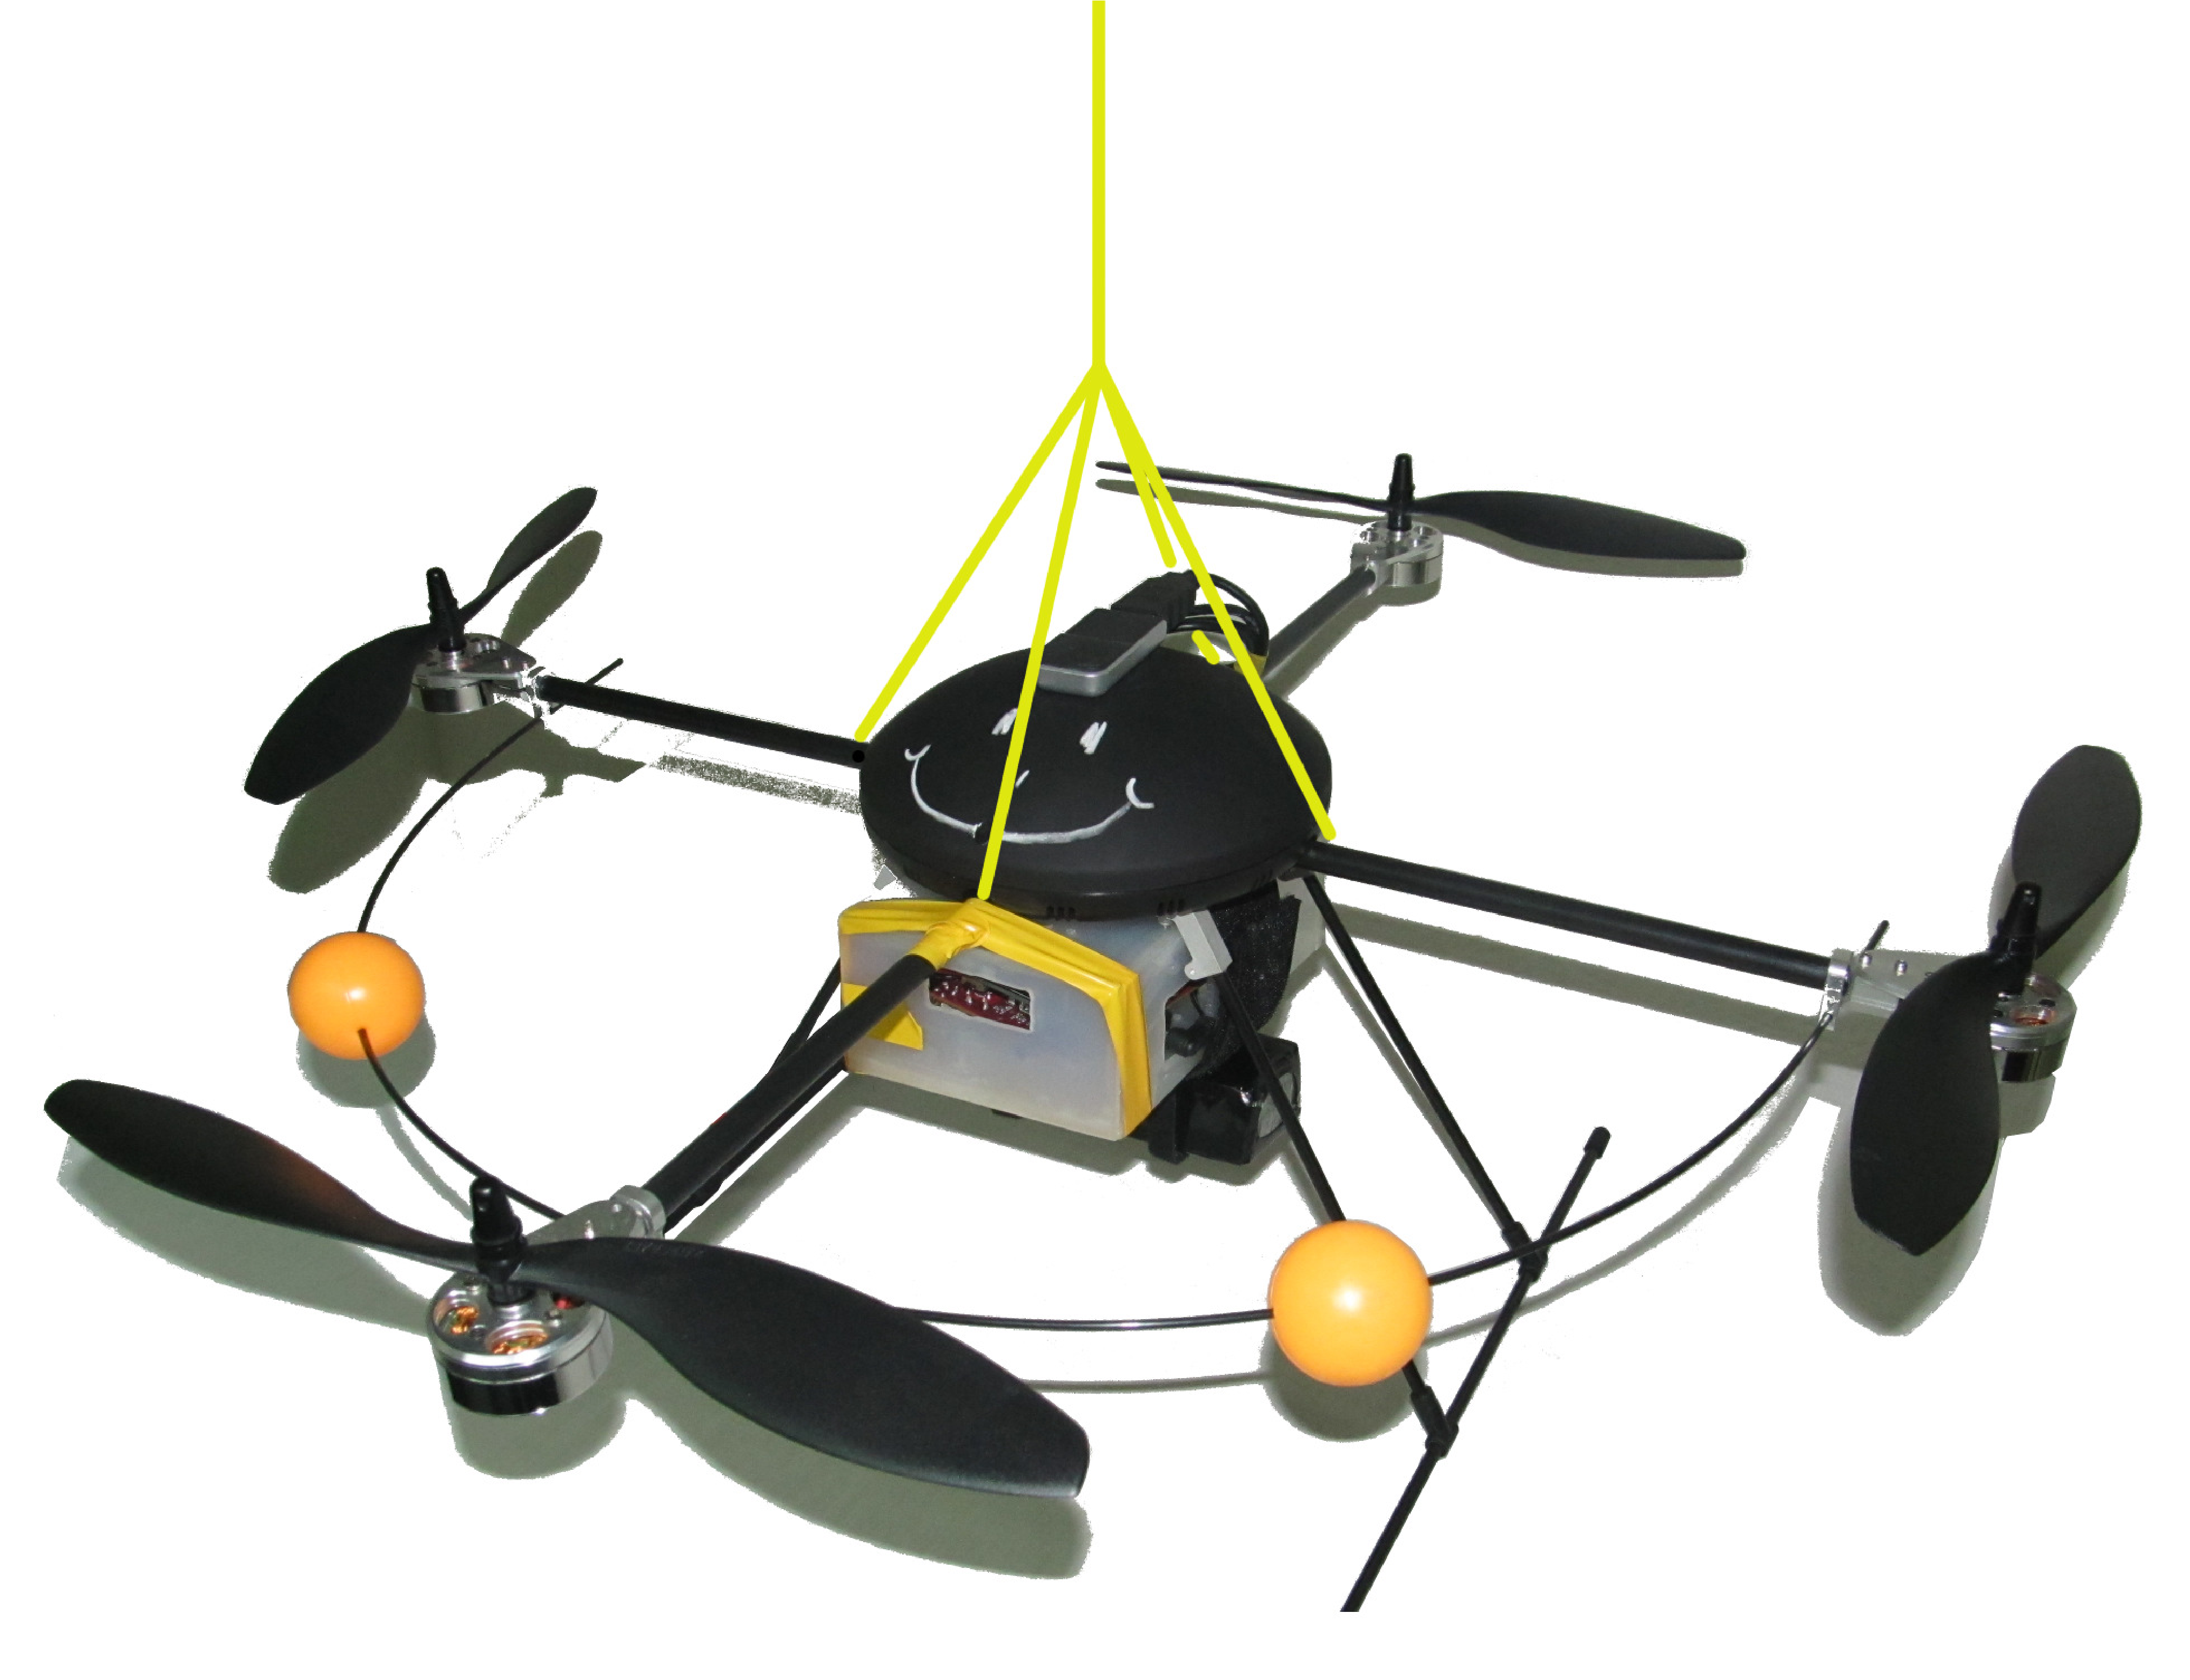
\includegraphics[width=0.4\textwidth]{./pics_test_control/dispositivo_theta.pdf}
	\caption{Dispositivo de prueba de $\theta$}
	\label{fig:thetadisp}
\end{wrapfigure}

El giro en $\theta$ es generado por un desequilibrio entre los pares ejercidos por las h\'elices. Si el par neto de todas las h\'elices resulta por ejemplo positivo, el cuadric\'optero realizar\'a un movimiento hacia los negativos, equilibrando el par, como se explica en el cap\'itulo \ref{chap:general}.\\

Para la estimaci\'on de $\theta$ se utiliza por un lado la integral de la velocidad angular en el eje ``z'' y por otro la proyecci\'on del vector del campo magn\'etico medido sobre el plano horizontal, medidas que son combinadas en el filtro de Kalman. El dato obtenido del magnet\'ometro no distingue entre giros de $360^o$, limitando el valor al rango [$-180^o$ - $180^o$]. Es necesario entonces realizar un reajuste de la medida deducida del campo magn\'etico para lograr la continuidad en el \'angulo estimado.\\

\end{document}